\documentclass[11pt,a4paper]{article}

\usepackage[T1]{fontenc}
\usepackage[utf8]{inputenc}
\usepackage{lmodern}
\usepackage[margin=1.15in]{geometry}
\usepackage{microtype}
\usepackage{amsmath,amssymb,amsthm,mathtools}
\usepackage{booktabs,longtable,tabularx,array}
\usepackage{graphicx}
\usepackage{xcolor}
\usepackage{tikz}
\usetikzlibrary{arrows.meta,positioning,calc,patterns,decorations.pathreplacing}
\usepackage[group-separator={,},group-minimum-digits=4]{siunitx}
\usepackage{algorithm}
\usepackage{algpseudocode}
\usepackage{enumitem}
\usepackage{caption}
\usepackage[hidelinks]{hyperref}
\usepackage[capitalise,noabbrev]{cleveref}
\usepackage{titlesec}
\usepackage{fancyhdr}

\setlist{itemsep=2pt,topsep=4pt,parsep=0pt}
\captionsetup{font=small,labelfont=bf,skip=6pt}
\titleformat{\section}{\large\bfseries}{\thesection}{0.7em}{}
\titleformat{\subsection}{\normalsize\bfseries}{\thesubsection}{0.7em}{}
\titleformat{\subsubsection}{\normalsize\itshape}{\thesubsubsection}{0.7em}{}
\renewcommand{\arraystretch}{1.12}
\setlength{\parindent}{1.2em}
\setlength{\parskip}{0pt}
\pagestyle{fancy}\fancyhf{}
\fancyhead[L]{\small\itshape Reverse-and-add of 196 on one laptop GPU}
\fancyhead[R]{\small Preprint, not peer reviewed}
\fancyfoot[C]{\small\thepage}
\renewcommand{\headrulewidth}{0.3pt}

\definecolor{accent}{HTML}{B8400A}
\newcommand{\code}[1]{\texttt{\small #1}}
\newcommand{\rev}{\operatorname{rev}}
\newcommand{\xor}{\oplus}
\newcommand{\Iverson}[1]{[\,#1\,]}
\newcommand{\gen}{G}
\newcommand{\prop}{P}
\newtheorem{proposition}{Proposition}
\newtheorem{lemma}[proposition]{Lemma}
\theoremstyle{remark}
\newtheorem{remark}{Remark}

\begin{document}

\begin{center}
{\Large\bfseries Exact reverse-and-add of 196 on a single laptop GPU:\\[2pt]
a bit-sliced, time-blocked engine and a run to 6.04 billion iterations\par}
\vspace{1.1em}
{\large taco-jpg}\\[2pt]
{\small Independent. \texttt{github.com/taco-jpg/p196-algorithm}}\\[2pt]
{\small 9 November 2026 \quad\textbullet\quad Preprint (draft), not peer reviewed}
\end{center}
\vspace{0.6em}

\begin{abstract}
\noindent
We describe an exact engine for the reverse-and-add map $N\mapsto N+\rev(N)$ iterated on $196$, its ten-version development history, and a production run that used it. The state of an $n$-digit number is its $\lceil n/2\rceil$ \emph{pair sums} $S_j=d_j+d_{n-1-j}$, stored as five bit-planes; one step is two carry chains, each a single binary integer addition per 32 pairs, plus a local update, and both the growth of the digit count and the palindrome test come from the same carries. Because a pair of the next number depends only on its neighbours and on runs of pair sums equal to $9$, a GPU thread block can advance a tile by up to 256 steps while tracking, at every step, the interval of pairs whose value is still \emph{certified} exact; any window whose interval fails to cover the block is restored and replayed by a slow exact per-step kernel. In the last version the pair sums are held in a decimal form whose update circuits were found by SAT and genetic search over 3-input logic gates. On one 6\,GB RTX~4050 laptop GPU (35--43\,W) the engine took the orbit from iteration \num{523226464} (\num{216579568} digits) to iteration \num{6040000000} (\num{2500134759} digits) in 27.6 days. No iterate computed in the run is a palindrome. The run was checked by certified arithmetic, a mod-9 fingerprint of every window, a mod-9 chain between archives (202 of 202 passed), a weekly recomputation by an independent kernel (4 of 4 passed), and agreement with the published value at iteration $10^9$. The note concerns computation only and makes no claim about what happens beyond the iterates computed.
\end{abstract}

\vspace{0.3em}
\noindent\textbf{Keywords:} reverse-and-add, 196 problem, Lychrel numbers, bit slicing, GPU, temporal blocking, exact arithmetic.

\section{Introduction}\label{sec:intro}

For a positive integer $N$ let $\rev(N)$ denote its decimal reversal. The \emph{reverse-and-add} map is $N\mapsto N+\rev(N)$. Starting from $N_0=196$ and setting $N_{t+1}=N_t+\rev(N_t)$, no palindromic $N_t$ has ever been found, although the question of whether one exists is open. The standard way of gathering evidence is to push $t$ as far as possible and to test every iterate; this quest goes back to at least the late 1980s~\cite{walker1990,p196org,oeis6960}. The digit count of $N_t$ grows by a nearly constant fraction of a digit per step (\cref{sec:run}: $0.4139$ digits per iteration), so the cost of one step grows linearly and the cost up to iteration $T$ grows like $T^2$.

\paragraph{Contributions.}
This note describes the machinery that made a run of several billion iterations feasible on a single consumer GPU, and the run itself.
\begin{itemize}
\item An exact formulation of one step in terms of pair sums, in which carries become binary integer additions and the digit growth and palindrome test fall out of the same carries (\cref{sec:pairs,sec:bits}).
\item A time-blocked GPU kernel in which each thread block advances a tile for many steps with no communication, justified by a \emph{certified interval} that is tracked exactly at every step; failures are repaired by exact replay, so correctness never depends on a probabilistic argument (\cref{sec:blocking}).
\item A decimal formulation of the pair sums inside register windows, with gate networks found by SAT and genetic search (\cref{sec:decimal}).
\item The ten-version lineage of the engine, with what each version changed and what was measured (\cref{sec:lineage}).
\item A layered verification scheme suited to a GPU without ECC memory (\cref{sec:verify}).
\item A $27.6$-day production run to \num{2500134759} digits, with its data and checkpoint hashes (\cref{sec:run}).
\end{itemize}

\paragraph{Scope.}
This note is about computation only. A computation shows what happens in finitely many steps; it does not say whether a palindrome ever appears, and nothing in it is used in an argument about all times. Nothing here is formally verified.

\section{One step in terms of pair sums}\label{sec:pairs}

Let $N$ have $n$ digits $d_{n-1}\cdots d_0$ and let $h=\lceil n/2\rceil$. Column $j$ of $N+\rev(N)$ adds $d_j+d_{n-1-j}$. This sum is the same for columns $j$ and $n-1-j$, so the addition is described by the \emph{pair sums}
\begin{equation}
S_j=d_j+d_{n-1-j},\qquad 0\le j<h,\qquad 0\le S_j\le 18,
\end{equation}
where for odd $n$ the middle pair is $2d_{\rm mid}$. Define the generate and propagate indicators
\begin{equation}
\gen_j=\Iverson{S_j\ge 10},\qquad \prop_j=\Iverson{S_j=9}.
\end{equation}
A pair sum of $9$ propagates an incoming carry ($9+1=10$), a pair sum $\ge10$ produces a carry whatever comes in, and a pair sum $\le 8$ absorbs it.

\paragraph{Carries.}
Let $a_j$ be the carry into low column $j$ and $b_j$ the carry into the mirrored high column $n-1-j$. Then
\begin{align}
a_0&=0, & a_{j+1}&=\gen_j\lor(\prop_j\land a_j),\\
b_{h-1}&=\begin{cases}a_h&n\text{ even}\\ a_{h-1}&n\text{ odd}\end{cases}, & b_{j-1}&=\gen_j\lor(\prop_j\land b_j).
\end{align}
The first recurrence moves carries up the low half, the second moves them down the pair index in the high half, and $b_{h-1}$ is the carry that crosses the middle. The carry out of the top column is $b_{-1}$; it is the \emph{growth bit} $g$, and $N+\rev(N)$ has $n+1$ digits if and only if $g=1$. Unwinding the recurrence shows that $g$ is the generate bit of the first pair, counted from the outside, whose sum is not $9$ (if every pair sum is $9$ the carry across the middle decides).

\paragraph{The next state.}
If $g=0$ the new pair sums are
\begin{equation}\label{eq:nogrowth}
S'_j=2S_j+a_j+b_j-10\,(a_{j+1}+b_{j-1}).
\end{equation}
If $g=1$ the number gains a digit. The low digit of new pair $j$ is $\mathrm{lo}_j=S_j+a_j-10a_{j+1}$, the high digit is the high digit of old pair $j-1$, $\mathrm{hi}_{j-1}=S_{j-1}+b_{j-1}-10b_{j-2}$, with $\mathrm{hi}_{-1}=1$ the new leading digit, and
\begin{equation}\label{eq:growth}
S'_j=\mathrm{lo}_j+\mathrm{hi}_{j-1}.
\end{equation}
(For even $n$ the new middle pair is $2\,\mathrm{hi}_{h-1}$.) These formulas are those of the reference implementation and were checked against schoolbook big-number arithmetic.

\begin{figure}[t]
\centering
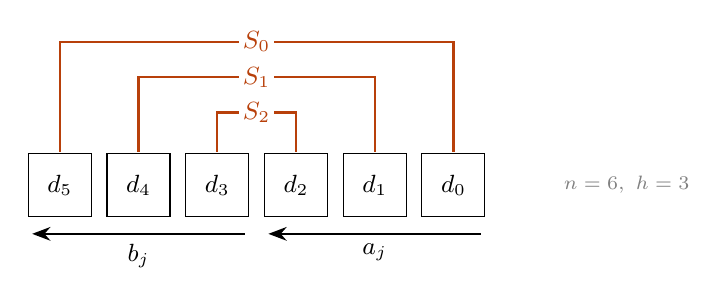
\begin{tikzpicture}[>=Stealth,font=\small]
 \foreach \i/\d in {0/d_{5},1/d_{4},2/d_{3},3/d_{2},4/d_{1},5/d_{0}}{
   \node[draw,minimum size=0.8cm] at (\i*1.0,0) {$\d$};
 }
 \foreach \i/\k/\h/\sj in {0/5/1.4/S_0,1/4/0.95/S_1,2/3/0.5/S_2}{
   \draw[accent,thick] (\i,0.42) -- (\i,0.42+\h) -- (\k,0.42+\h) -- (\k,0.42);
   \node[accent,fill=white,inner sep=1.5pt] at (2.5,0.42+\h) {$\sj$};
 }
 \draw[->,thick] (5.35,-0.62) -- (2.65,-0.62) node[midway,below] {$a_j$};
 \draw[->,thick] (2.35,-0.62) -- (-0.35,-0.62) node[midway,below] {$b_j$};
 \node[font=\scriptsize,gray] at (7.2,0) {$n=6,\ h=3$};
\end{tikzpicture}
\caption{Folding. Digits $d_j$ and $d_{n-1-j}$ are added in the same two columns of $N+\rev(N)$, so $N+\rev(N)$ is described by the $h=\lceil n/2\rceil$ pair sums $S_j$. Carries $a_j$ run up the low half (right to left in the written number, pair index increasing) and carries $b_j$ run through the high half towards the outside (pair index decreasing).}
\label{fig:fold}
\end{figure}

\paragraph{Palindrome test.}
$N_{t+1}$ is a palindrome iff its low digit $j$ equals its high digit $j$ for every $j$. In terms of the same quantities: if $g=0$ this is $a_j=b_j$ for all $j$ (the difference of the two digits is $(a_j-b_j)-10(a_{j+1}-b_{j-1})$, which can vanish only if both brackets do); if $g=1$ it is $\mathrm{lo}_j=\mathrm{hi}_{j-1}$ for all $j$. The test costs one XOR per word, and each iterate is tested exactly once, in the step that produces it.

\paragraph{Digit sums.}
$\rev(x)$ has the digit sum of $x$, hence
\begin{equation}\label{eq:mod9}
x+\rev(x)\equiv 2x\pmod 9\quad\text{for every }x,
\end{equation}
which is used for checking in \cref{sec:verify}.

\paragraph{A worked step.}
Take $N=1675$ ($n=4$, $h=2$): $S_0=5+1=6$ and $S_1=7+6=13$, so $\gen=(0,1)$ and $\prop=(0,0)$. Then $a_0=0$, $a_1=0$, $a_2=1$, $b_1=a_2=1$, $b_0=\gen_1=1$, and $g=b_{-1}=\gen_0\lor(\prop_0\land b_0)=0$, so there is no growth. By \eqref{eq:nogrowth}, $S'_0=12+0+1-10(0+0)=13$ and $S'_1=26+0+1-10(1+1)=7$. Directly, $1675+5761=7436$ and $7+6=13$, $4+3=7$. \qed

\section{Bit-sliced state}\label{sec:bits}

The state is the $h$ pair sums, five bits each, stored as five bit-planes of 32-bit words: word $k$ of plane $q$ holds bit $q$ of $S_{32k},\dots,S_{32k+31}$. At $2.5\times10^9$ digits this is $5\times1.25\times10^9$ bits, $0.78$\,GB. The GPU memory in use at $2.47\times10^9$ digits was $2.38$\,GiB, consistent with three copies of the state (current, next, and a backup for replay) plus working space; this is why a 6\,GB card suffices.

\paragraph{Carries as integer additions.}
For one word put $X=\gen\lor\prop$ (carry-capable pairs). Since $\prop$ and $\gen$ are disjoint, $X_j\land\gen_j=\gen_j$ and $X_j\xor\gen_j=\prop_j$. The carry out of bit $j$ of the integer addition $X+\gen+c_{\rm in}$ is the majority of $X_j,\gen_j$ and the carry into bit $j$, i.e.\ $\gen_j\lor(\prop_j\land c_j)$, which is exactly the recurrence of \cref{sec:pairs}. So the 32 carries into a word are
\begin{equation}
a=(X+\gen+c_{\rm in})\xor X\xor\gen,
\end{equation}
and the carry out of the word is the carry out of that addition. The high chain is the same addition on bit-reversed words. \Cref{alg:carry} gives the whole word-level computation.

\begin{algorithm}[t]
\caption{Carries of one 32-pair word (low chain; the high chain is the same on bit-reversed planes).}\label{alg:carry}
\begin{algorithmic}[1]
\Require planes $S^{(4)},\dots,S^{(0)}$ of the word, carry-in $c_{\rm in}\in\{0,1\}$
\State $\gen\gets S^{(4)}\lor\bigl(S^{(3)}\land(S^{(2)}\lor S^{(1)})\bigr)$ \Comment{$S\ge10$}
\State $\prop\gets\lnot S^{(4)}\land S^{(3)}\land\lnot S^{(2)}\land\lnot S^{(1)}\land S^{(0)}$ \Comment{$S=9$}
\State $X\gets\gen\lor\prop$
\State $s\gets X+\gen+c_{\rm in}$ \Comment{one 33-bit integer addition}
\State $a\gets s\xor X\xor\gen$ \Comment{carry \emph{into} each of the 32 pairs}
\State $c_{\rm out}\gets$ carry out of the addition
\State \Return $a,\;c_{\rm out}$
\end{algorithmic}
\end{algorithm}

Carries between words are resolved by scanning for the nearest word that is not ``all propagate'' (all 32 pairs equal to $9$, probability about $10^{-32}$ per word on digit data that look random), so the arithmetic is exact with no cutoff.

\section{Time blocking with certified windows}\label{sec:blocking}

A step touches every word, so a naive GPU implementation streams the whole state from memory each step. The engine instead lets each thread block keep a \emph{tile} of the state on chip and advance it by many steps. The idea is that of temporal blocking with redundant ``ghost-zone'' computation in stencil codes~\cite{frigo2005,meng2009}; here the dependence is data-dependent (carry chains), so the extent of the valid region is tracked at run time rather than fixed in advance.

\paragraph{Locality and the certified interval.}
Pair $j$ of the next state depends on pairs $j-1,j,j+1$ and, through a carry chain, on the run of $9$-pairs next to them. Suppose the values on pairs $[L,R)$ of a tile are exact and nothing is known outside. After one step the values are exact on $[L',R')$ with
\begin{align}\label{eq:interval}
L'&=\bigl(\text{first pair}\ge L\text{ whose sum is not }9\bigr)+1,\notag\\
R'&=\bigl(\text{last pair}<R\text{ whose sum is not }9\bigr)+g,
\end{align}
because the carry past a non-$9$ pair no longer depends on the unknown side. (At the outer end of the number $L=0$ stays $0$; in the middle the interval is anchored by the carry across the centre.) For digit data that look random a pair sum is $9$ with probability $0.1$, so each edge moves about $1.1$ pairs per step; $64$ steps move an edge by about $71$ pairs (\cref{fig:interval}). The interval is tracked at every step. No approximation or probabilistic argument is involved: long carry chains cost replays, never correctness.

\begin{figure}[t]
\centering
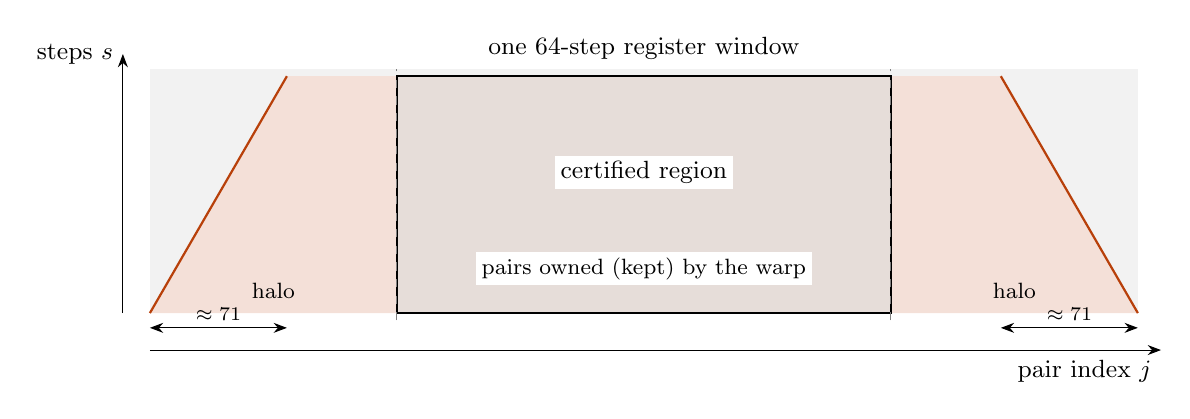
\begin{tikzpicture}[x=0.0245cm,y=0.047cm,>=Stealth,font=\small]
 \fill[black!5] (0,0) rectangle (512,66);
 \fill[accent!16] (0,0) -- (512,0) -- (441,64) -- (71,64) -- cycle;
 \draw[accent,thick] (0,0) -- (71,64);
 \draw[accent,thick] (512,0) -- (441,64);
 \draw[thick,fill=black!14,fill opacity=0.55] (128,0) rectangle (384,64);
 \draw[dashed,gray] (128,-2) -- (128,66);
 \draw[dashed,gray] (384,-2) -- (384,66);
 \draw[->] (-14,0) -- (-14,70) node[left] {steps $s$};
 \draw[->] (0,-10) -- (524,-10) node[below left] {pair index $j$};
 \node[above] at (256,66) {one 64-step register window};
 \node[fill=white,inner sep=2pt] at (256,38) {certified region};
 \node[fill=white,inner sep=2pt,font=\footnotesize] at (256,12) {pairs owned (kept) by the warp};
 \node[font=\footnotesize,align=center] at (64,6) {halo};
 \node[font=\footnotesize,align=center] at (448,6) {halo};
 \draw[<->] (0,-4) -- (71,-4) node[midway,above=-1pt,font=\scriptsize] {$\approx71$};
 \draw[<->] (441,-4) -- (512,-4) node[midway,above=-1pt,font=\scriptsize] {$\approx71$};
\end{tikzpicture}
\caption{A register window (owned width not to scale). The certified interval (red) shrinks by about $1.1$ pairs per step at each edge; the window is accepted only if, after its last step, it still covers every pair the warp owns (grey); the halo of 128 pairs on each side absorbs the shrinkage. Otherwise the window is restored from its backup and replayed by the exact per-step kernel.}
\label{fig:interval}
\end{figure}

\paragraph{Growth tape.}
The growth bit of each step depends only on the outermost pairs. Before every launch of $K$ steps, a small kernel runs the prefix of the number alone and writes $g_0,\dots,g_{K-1}$, certified by the same interval rule, so thread blocks never wait for each other during the launch. Production used $K=256$.

\paragraph{Three nested units and exact replay.}
A \emph{launch} is $K=256$ steps on a tile. Inside a launch each block (version v8 and later) works in \emph{register windows} of up to $64$ steps: it loads its pairs plus a halo of unverified pairs, runs the window alone, and at the end compares the certified interval with the pairs it owns. The driver groups launches into \emph{verification windows} of \num{8192} steps. If in a verification window any owned pair is not certified, any palindrome flag is raised, or the fingerprint of \cref{sec:verify} fails, the window is restored from its backup and replayed by the slow, exact per-step kernel (v4), which resolves every carry by full scans. Production recorded two such replays in \num{5518} chunks of $10^6$ steps; neither was a fingerprint mismatch. Results are therefore bit-identical to the schoolbook computation whether or not a window is replayed.

\paragraph{Warp windows (v9).}
The 32 lanes of a warp share a register window and pass the carries that cross lane boundaries with warp shuffles, which run on a different unit from the integer ALU: 32 groups of four words are loaded and 30 kept, instead of recomputing a halo word per thread.

\section{Decimal pair sums in registers (v10)}\label{sec:decimal}

In v9 each step converted pair sums to carries with a 5-plane addition and subtraction. In v10 a window keeps each pair sum as $S=D+10G$, with $D=S\bmod 10$ in four binary-coded-decimal planes and $G=\Iverson{S\ge10}$ in one. Then $G$ and $P=\Iverson{D=9}$ are exactly the carry generate and propagate planes, and the new pair sum depends only on the carries into the pair:
\begin{itemize}
\item no growth: $D'=(2D+c)\bmod 10$ with $c=a_j+b_j$, and $G'=\Iverson{D+(a_j\land b_j)\ge5}\land\lnot\bigl(P\land(a_j\lor b_j)\bigr)$;
\item growth: a BCD addition $D_j+a_j+\mathrm{hi}_{j-1}$ whose high digit is produced in excess-6 form, so the decimal carry is the binary carry out of bit 3.
\end{itemize}
The gate networks (3-input LOP3 gates~\cite{ptx}, one instruction each) were found by exact SAT synthesis~\cite{kojevnikov2009} for single outputs and by Cartesian genetic programming~\cite{miller2000} for multi-output functions, and checked exhaustively (\num{5246400} cases). A word's no-growth update costs $10$ gates (v9: about $29$). The static instruction counts of the step loop (compiler output, not measured) fall from about $220$ ALU-pipe instructions per lane-step in v9 to about $96$ in v10. Conversion between binary planes and $(D,G)$ happens only when a window is loaded or stored, so tiles, checkpoints and the other kernels are unchanged.

\section{Engine lineage, v1 to v10}\label{sec:lineage}

The engine was developed in ten numbered generations, with several intermediate variants (v5\,diag, v6s, v6r, v6r2, v6r3, v7r, v8b). Every release keeps the same command line, checkpoint format and result: from v4 on the output of each version is byte-identical to the previous one, which, from v6 on, was enforced by a differential test before it could replace it. \Cref{tab:lineage} lists what each generation changed and the evidence in its release notes; \cref{sec:run} gives the production measurements for the five versions that actually ran the orbit. Two caveats: the per-version figures in \cref{tab:lineage} were measured by different people at different times on different inputs (noted per row), and several speed estimates in the release notes were made before a GPU run and turned out too optimistic; the notes themselves say so.

\begingroup\small
\setlength{\tabcolsep}{4pt}
\begin{longtable}{@{}p{0.075\linewidth}p{0.50\linewidth}p{0.34\linewidth}@{}}
\caption{The ten generations of the engine. ``Prod.'' marks versions that ran the production orbit (\cref{tab:engines}). All figures are from the release notes of the version named, except the production figures.}\label{tab:lineage}\\
\toprule
Version & What changed & Evidence / outcome\\
\midrule
\endfirsthead
\toprule
Version & What changed & Evidence / outcome\\
\midrule
\endhead
\bottomrule
\endfoot
v1, v2 & Early prototypes before the archived release series. & Not described or used here.\\
v3 & First archived release. Folded pair sums $S_j$ with exact carries computed by each thread scanning the input prefix for the nearest non-$9$ pair (no truncation). CUDA graphs of 32 steps per submission, GPU palindrome flag, resumable decimal checkpoints, chunked driver. A Metal version is kept for comparison. & 20\,000 steps on \num{2046548} digits: 0.83\,s CUDA vs.\ 1.21\,s Metal on the user's RTX~4050 and M1 Max (reported). CPU: 4.8\,ms per step at that size.\\
v4 & \textbf{Bit slicing.} Five bit-planes, carries as integer additions (\cref{sec:bits}), growth and palindrome from the same carries; one 32-bit instruction handles 32 pairs. Also the exact per-step kernel used ever after for replay. & GPU time for the same 20\,000 steps: 0.082\,s vs.\ 0.770\,s for the v3 kernel ($4.1\ \mu$s per step, $9.4\times$). CPU emulation: $14\times$ less work per step.\\
v5 & \textbf{Time blocking.} Tiles in shared memory advanced $K$ steps per launch; certified interval; growth bits from a prefix tile in every block; failure repaired by v4 replay of the verification window. \emph{Run mode}: one persistent process, background checkpoint writer, \code{latest.json}, newest-3 retention. & Exactness suite (small numbers, adversarial $9$-runs, delayed palindromes at 24, 55 and 261 steps) and a soundness checker with zero violations on the CPU emulator. The production engine before v6r2 (the v6 diagnostic notes say production stays on v5).\\
v5\,diag, v6, v6s & v6: ``lean'' time-blocked kernel. v5\,diag: phase profiler (track / work / barrier cycles per step). v6s: v6 with a compiler defect fixed (rare-path functions took arrays by reference and forced a 168-byte local-memory frame on the hot path). & v6 was \emph{slower} than v5: 28M digits 55.0 vs.\ 52.3 $\mu$s per step; 2.05M digits 5.54 vs.\ 4.04 $\mu$s per step. The profile showed warp~0 (growth bit and tracking) on the critical path.\\
v6r, v6r2 & Rebalanced roles; v6r2: one inlined copy of the fast path, growth bit kept in registers. & Reported $1.48\times$ (v6r) and $1.10\times$ (v6r2) over the predecessor. \textbf{v6r2 (Prod.)} starts the run.\\
v6r3 & Nsight Compute profile (DRAM 1.8\% and L2 0.7\% busy: not memory bound; 51\% of scheduler cycles had no ready warp; per-step barrier the top stall; the card pinned at its 35\,W cap at about 1.9\,GHz). Tile geometry in registers, growth bit through the barrier, palindrome vote off the barrier, wider tiles (860 words). & \textbf{v6r3 (Prod.)}. Byte-identical to v6r2 (120/120 differential).\\
v7, v7r & \textbf{Transposed tiles}: word $u$, bit $k$ holds pair $P_0+k\,W_t+u$, so each lane owns a contiguous run and the carry chains run along the word index with one 3-input logic op per word, with no 64-bit adds and no bit reversal. v7r keeps this at four words per thread with halo lanes and register trackers. & v7: about $2\times$ fewer instructions per word, but half the resident warps per SM (IPC 0.7 vs.\ 2.7): measured $0.69\times$, not adopted. v7r: the notes report no GPU measurement; not used in production.\\
v8 & \textbf{Control tape and register micro-windows} (idea from an external review): a separate kernel writes the growth bits for a launch; each thread runs 8 steps on its own group plus a halo with no barrier or shared memory, certified per thread. Barriers per 128-step launch fall from 128 to 16; arithmetic rises $1.5\times$ because of the halo. & \textbf{v8 (Prod.)}.\\
v8b & 64-bit digit counts (the 32-bit count would have stopped the run at $2.147\times10^9$ digits; pair indices stay 32-bit, limit about $4.29\times10^9$ digits), 288 threads, any window length, optional base-5 window arithmetic, tools: ISF writer, mod-9 checker, weekly cross-check. & Production engine label was never \code{v8b}: v9 contained the same changes and replaced v8 before the limit mattered.\\
v9 & \textbf{Warp windows} (\cref{sec:blocking}): 30 of 32 lanes kept per warp, 128-pair halo, 64-bit carry chains on the ALU, shuffles for lane-edge carries, 4 barriers per 128-step launch, optional pipe balancing (shifts as multiply-adds), \emph{per-window mod-9 fingerprint}. & \textbf{v9 (Prod.)}. Static ALU instructions per lane-step about 225 vs.\ about 384 for v8b.\\
v10 & \textbf{Decimal pair sums} (\cref{sec:decimal}): BCD digit planes plus carry-generate plane; 10-gate update; windows of 64 steps; cheaper tracker and palindrome bookkeeping; slow per-step tiles scheduled first in each launch. & \textbf{v10 (Prod.)} from iteration $2.49\times10^9$; $1.7\times$ v9, size-normalised (\cref{tab:boundary}).\\
\end{longtable}
\endgroup

\paragraph{What the lineage shows.}
The first order-of-magnitude gain came from the representation (v3$\to$v4: bit slicing, $9.4\times$ on the GPU), the next from avoiding memory traffic and launch overhead with exactly tracked time blocking (v5). After that, profiling drove the changes: v6 was slower than v5 until a profile exposed a compiler artefact, v7 halved the instruction count and still lost because it halved the warps, and the largest later gains (v9, v10) came from removing redundant halo computation and then shrinking the logic of the step itself. The profile-before-guess habit was the main lesson: several predicted speed-ups were too high by a factor of two or more.

\section{Checking a long run on hardware without ECC}\label{sec:verify}

The card has no ECC memory, so a flipped bit is a real possibility over weeks. The run uses five independent layers.
\begin{enumerate}[leftmargin=1.6em]
\item \textbf{Exactness by construction.} Certification and exact replay (\cref{sec:blocking}). A CPU emulator compiles the very same kernel headers, so its gate (every certified block recomputed through the exact path; stress tests with planted $9$-runs; growth edge cases; a differential v9-versus-v10 test of 120 inputs; the 2-million-digit checkpoint advanced by \num{2000} steps in every configuration, equal to the schoolbook reference) tests the arithmetic that runs on the GPU. From v9 on, the emulator executes the 32 lanes of a warp as cooperating fibers, so shuffles and votes are exercised too.
\item \textbf{Mod-9 fingerprint of every window.} With $E_t=x_{t+1}\bmod 9$ computed from the pair sums as $2\sum_jS_j-\Iverson{n\text{ odd}}\,S_{\rm mid}\pmod 9$, identity \eqref{eq:mod9} requires $E_{t+m}\equiv 2^mE_t\pmod 9$. A single flipped bit in a state plane changes the digit sum by $\pm2^{q+1}$ (or $\pm2^q$ for the middle pair of an odd number), never a multiple of $9$, and later steps only multiply the discrepancy by powers of $2$, so any single flipped state bit is detected. A mismatch after a time-blocked window triggers the exact replay; a mismatch after the per-step kernel stops the run. Over the run no fingerprint replay occurred.
\item \textbf{Archive chain.} Every $25\times10^6$ iterations the checkpoint is compressed, read back and its digit SHA-256 compared, and the mod-9 identity between consecutive archives is checked on the digit strings themselves: 202 of 202 passed (iterations \num{975226464} to \num{6025000000}). The three checkpoints kept at the end (iterations \num{6038000000}, \num{6039000000}, \num{6040000000}) also satisfy the identity pairwise (digit sums $1,7,4$ mod $9$; each step of $10^6$ iterations multiplies by $2^{10^6}\equiv7$).
\item \textbf{Weekly independent recomputation.} Once a week (four times) $10^6$ steps were recomputed from a saved production checkpoint with the per-step reference kernel (a different code path, 3.8--8.8\,ms per step against 0.3--0.7\,ms for production); the result had to equal the production checkpoint byte for byte. 4 of 4 passed (from iterations \num{2083000000}, \num{3594000000}, \num{4895000000}, \num{5922000000}).
\item \textbf{External reference.} At iteration $10^9$ the digit count (\num{413930770}) and the 25 leading digits (\code{3932472453326071578739224}) equal the published values~\cite{p196org}; the checkpoint was also converted to the ISF format used by that site (CRC-16 header, 70 digits per line).
\end{enumerate}

\section{The production run}\label{sec:run}

\subsection{Setup}
\begin{itemize}
\item Hardware: one NVIDIA GeForce RTX~4050 Laptop GPU (Ada, \code{sm\_89}, 20 SMs, 6\,GB, no ECC) with a 13th-generation Core i7 host and 30\,GB of RAM. The card was power-limited at about 35\,W early in the run; from iteration about $3.70\times10^9$ it ran at about 43\,W (see below).
\item Final configuration: v10, 512 threads per block, 64-step register windows, $K=256$, tile 1892 words (\num{60544} pairs), verification windows of \num{8192} steps, checkpoint every $10^6$ iterations, three live checkpoints kept. A supervisor restarts the engine from the newest checkpoint and records one observation per checkpoint.
\item Start: a checkpoint at iteration \num{523226464} (\num{216579568} digits) from an earlier engine generation. This note does not rely on its provenance beyond the agreement at iteration $10^9$ (\cref{sec:verify}). Start 2026-10-12 21:05 UTC; stop 2026-11-09 10:39 UTC.
\end{itemize}

\subsection{Engines in production}

The engine was upgraded in place at checkpoint boundaries while the run continued; the results of each generation were required to be identical to the previous one. Medians are over chunks in which the board drew more than 30\,W (this excludes chunks that overlapped a pause). \emph{Digit-steps per second} is the product of steps per second and the digit count; since the work per step is proportional to $n$, it is the size-independent measure of engine speed.

\begin{table}[t]
\centering\small
\setlength{\tabcolsep}{4.5pt}
\caption{Engines that ran the production orbit.}\label{tab:engines}
\begin{tabular}{@{}lrrrrr@{}}
\toprule
Engine & Iterations ($10^6$) & Digits ($10^6$) & Chunks & Median steps/s & Median digit-steps/s ($10^{12}$)\\
\midrule
v6r2 & 523.2--618.2 & 216.6--255.9 & 89 & \num{4636} & 1.09\\
v6r3 & 619.2--669.2 & 256.3--277.0 & 48 & \num{4893} & 1.30\\
v8 & 670.2--980.2 & 277.4--405.7 & 308 & \num{4769} & 1.62\\
v9 & 981.2--2489 & 406.2--1030.3 & 1492 & \num{2851} & 2.04\\
v10 & 2490--6040 & 1030.7--2500.1 & 3513 & \num{2219} & 3.82\\
\bottomrule
\end{tabular}
\end{table}

\begin{table}[t]
\centering\small
\caption{Speed before and after each engine switch: median digit-steps per second ($10^{12}$) over the 40 chunks on each side. These are consecutive stretches of the same run, not controlled A/B tests; the digit count grows by 2--7\% across each boundary, and the card was in its early 35\,W state on both sides of every switch.}\label{tab:boundary}
\begin{tabular}{@{}lrrr@{}}
\toprule
Switch & Before & After & Ratio\\
\midrule
v6r2$\to$v6r3 & 1.09 & 1.30 & 1.20\\
v6r3$\to$v8 & 1.30 & 1.63 & 1.25\\
v8$\to$v9 & 1.58 & 2.04 & 1.29\\
v9$\to$v10 & 1.99 & 3.45 & 1.73\\
\bottomrule
\end{tabular}
\end{table}

The v9$\to$v10 ratio of $1.7$ ($1.68$ with 160 chunks on each side) lies in the $1.4$--$1.9$ range predicted from the instruction counts of \cref{sec:decimal}.

\subsection{Throughput and growth}

\Cref{fig:throughput}(a) shows steps per second falling as the number grows (the work per step is proportional to $n$); panel (b) shows that, normalised by size, each engine is flat and each switch is a step up. Within v10, panel (b) shows one further step of about $13\%$ near iteration $3.70\times10^9$. The engine did not change there. The logged median SM clock changes from \num{1708}\,MHz (iterations $2.49$--$3.69\times10^9$) to \num{1929}\,MHz (from $3.72\times10^9$), board power from 35.0 to 43.3\,W and temperature from 69 to 82\,$^\circ$C; the v6r3 profile had recorded the card pinned at its 35\,W software cap. The cause of the change of state is outside the engine and was not investigated.

\begin{figure}[t]
\centering
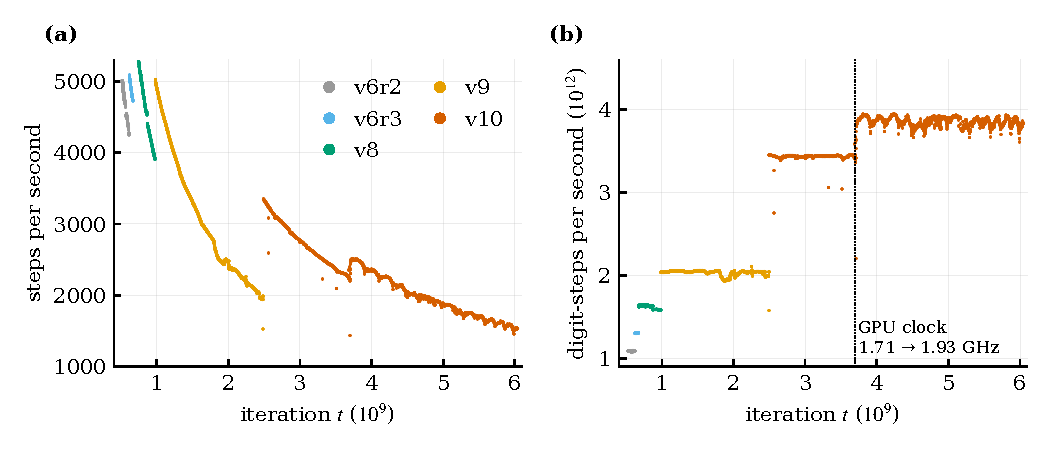
\includegraphics[width=\linewidth]{figs/fig_throughput.pdf}
\caption{Per-chunk throughput over the run (chunks with board power above 30\,W), coloured by engine. (a) Steps per second. (b) Digit-steps per second ($10^{12}$). The dotted line marks the change of GPU clock and power state near iteration $3.70\times10^9$.}
\label{fig:throughput}
\end{figure}

\begin{figure}[t]
\centering
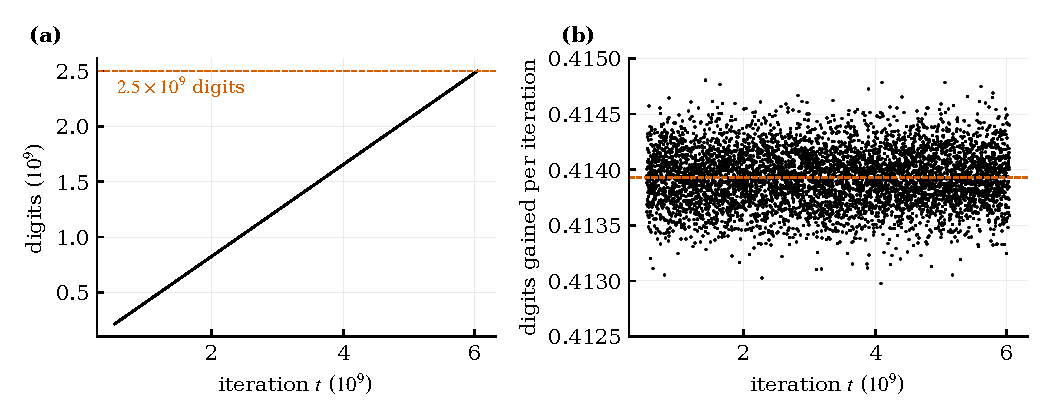
\includegraphics[width=\linewidth]{figs/fig_growth.pdf}
\caption{Digit count of the iterates. (a) Digits against iteration. (b) Digits gained per iteration, one point per chunk of $10^6$ iterations; the dashed line is the run average, $0.41393$ digits per iteration (standard deviation of the chunk values $2.5\times10^{-4}$).}
\label{fig:growth}
\end{figure}

\begin{table}[t]
\centering\small
\caption{Throughput at selected iterations (one chunk each).}\label{tab:throughput}
\begin{tabular}{@{}rrrr@{}}
\toprule
Iteration & Digits & Steps/s & $\mu$s per step\\
\midrule
\num{2490000000} & \num{1030678354} & \num{3349} & 297\\
\num{3000000000} & \num{1241792914} & \num{2758} & 361\\
\num{4000000000} & \num{1655710949} & \num{2370} & 420\\
\num{5000000000} & \num{2069641916} & \num{1871} & 532\\
\num{5977000000} & \num{2474055055} & \num{1512} & 658\\
\num{6040000000} & \num{2500134759} & \num{1535} & 648\\
\bottomrule
\end{tabular}
\end{table}

Over the whole run the digit count grew by $0.41393$ digits per iteration; the last chunk before the stop added \num{413593} digits for $10^6$ iterations. At $2.5\times10^9$ digits one step takes $648\ \mu$s, about $3.8\times10^{12}$ digit-steps per second. In total the run performed about $3.7\times10^{18}$ pair updates (about $0.1035\,(T^2-T_0^2)$ with $T=6.04\times10^9$ and $T_0=523\,226\,464$).

\subsection{Checkpoint hashes}
The file \code{paper/data/milestones.csv} of the repository lists the digit count and the SHA-256 of the digit string (no header, no newline) of the checkpoint at every multiple of $5\times10^8$ iterations from $10^9$ to $5.5\times10^9$, and of the final checkpoint; \code{paper/data/throughput.csv} gives the per-chunk data behind \cref{fig:throughput,fig:growth}. For example, at iteration $10^9$: \num{413930770} digits, SHA-256 \code{e2418907e5be1f4b3b74a11d904f3e7b069022d0cbd6cdefc1cefc890c822365}. The digit files (2--3\,GB each) are not stored in the repository.

\subsection{Result}
The run stopped on request at the first checkpoint with at least $2.5\times10^9$ digits: iteration \num{6040000000}, with \num{2500134759} digits, on 2026-11-09 at 10:39 UTC, 27.6 days after the start. The leading 25 digits are \code{1712328959881746707154772}, the trailing 25 digits are \code{5187460706747189948933117}, and the SHA-256 of the digit string is
\begin{center}\code{256b41db46da72891caae69cf51fd9c52a2e5cbe3a6ad804ebd8de0d55b177a9}.\end{center}
The number is not a palindrome. No window needed a fingerprint replay, two windows needed a certification replay, and all archive, weekly and external checks of \cref{sec:verify} passed. This is the end of a finite computation: it says nothing about iterations beyond \num{6040000000}.

\section{Limits and costs}\label{sec:limits}
\begin{itemize}
\item Pair indices are 32-bit, so the engine handles $n<4.29\times10^9$ digits. Three state copies at that size take about 4\,GB, within the 6\,GB of the card.
\item Time per step grows linearly with $n$. Reaching $4\times10^9$ digits needs iteration $\approx9.7\times10^9$; extrapolating the measured $3.8\times10^{12}$ digit-steps per second, that is about five to six more weeks on this card (an extrapolation, not a measurement).
\item The fingerprint catches any single flip per window, not every multi-bit corruption; the weekly recomputation and the archive chain are the backstop. Neither of them can prove the absence of an error that cancelled in all of them.
\item Everything above concerns the finitely many iterates computed.
\end{itemize}

\section{Reproducing}\label{sec:repro}
The sources of every generation are in the \code{calculation/} directory of the repository (one archive per release; v10 is \code{lychrel196\_v10.zip}). A run from the checkpoint shipped in the archive:
\begin{verbatim}
unzip calculation/lychrel196_v10.zip && cd lychrel196_v10
nvcc -O3 -std=c++17 -arch=sm_89 cuda196_v10.cu -o cuda196_v10
./cuda196_v10 run checkpoint_4942464.txt 4942464 out \
    --chunk=1000000 --keep=3 --K=256 --tile=1892
cc -O2 tools/mod9.c -o mod9 && ./mod9 A.txt IT_A B.txt IT_B
./bench_v10.sh gate     # CPU-emulator gate and GPU exactness suites
\end{verbatim}
\code{tools/ref.c} is the schoolbook reference, \code{tools/crosscheck.sh} the weekly independent recomputation, \code{tools/isf.c} the ISF writer, and \code{synth/} reproduces the gate networks.

\section*{Acknowledgements}
The text and figures of this note were prepared with the assistance of an AI model (Claude, Anthropic); the author is responsible for its content.

\begin{thebibliography}{99}\small
\bibitem{walker1990} J.~Walker, \emph{Three Years of Computing: Final Report on the 196 Palindrome Quest}, 1990 (Fourmilab).
\bibitem{p196org} p196.org: the 196 palindrome quest, history and records (record at iteration $10^9$, \num{413930770} digits, news page dated 2011-12-27).
\bibitem{oeis6960} OEIS A006960: ``Reverse and Add! trajectory of 196''.
\bibitem{frigo2005} M.~Frigo and V.~Strumpen, Cache oblivious stencil computations, in \emph{Proc.\ 19th ACM Int.\ Conf.\ on Supercomputing (ICS)}, 2005, pp.~361--366.
\bibitem{meng2009} J.~Meng and K.~Skadron, Performance modeling and automatic ghost zone optimization for iterative stencil loops on GPUs, in \emph{Proc.\ 23rd Int.\ Conf.\ on Supercomputing (ICS)}, 2009, pp.~256--265.
\bibitem{kojevnikov2009} A.~Kojevnikov, A.\,S.~Kulikov and G.~Yaroslavtsev, Finding efficient circuits using SAT-solvers, in \emph{SAT 2009}, LNCS 5584, 2009, pp.~32--44.
\bibitem{miller2000} J.\,F.~Miller and P.~Thomson, Cartesian genetic programming, in \emph{EuroGP 2000}, LNCS 1802, 2000, pp.~121--132.
\bibitem{ptx} NVIDIA, \emph{Parallel Thread Execution ISA}, instruction \code{lop3}.
\end{thebibliography}

\end{document}
